\documentclass[12pt, a4paper]{article}
 

\usepackage{graphicx}
\graphicspath{ {./images/} }
%Tarih Ekleme
\usepackage[ddmmyyyy]{datetime}
\renewcommand{\dateseparator}{.}
\renewcommand{\figurename}{Şekil}
\renewcommand{\refname}{Kaynaça}




\title{Metinden görsel oluşturma projesi}
\author{Mustafa Erdoğdu}
\date{\today}
%\date{\DTMnow}
%\date{\DTMnow}


\begin{document}
	
			
			\begin{figure}[h]
				\centering
				
\includegraphics{ksbu.png}
			\end{figure}
			\maketitle
			\thispagestyle{empty}
			
		

			\section{Giriş}		
			Bu rapor, "Metinden görsel üretme" adlı projenin detaylarını içermektedir
			Projenin temel amacı, metinden görsel üretebilen bir yapay zeka modeli geliştirebilmektir.
			Hedef, kullanıcı tarafından oluşturulan doğa tasvirini derin öğrenme yöntemleri kullanarak özgün ve yaratıcı doğa görselleri oluşturabilen bir sistem oluşturmaktır.
			
			\section{Literatür Araştırması}
			
				\textbf{Kullanılan ve Benzer çalışmalar}
			
			\subsection{Nlp(doğal dil işleme)}		
			Doğal dil işleme (NLP), bilgisayarlara insan dilini yorumlama, işleme ve anlama yeteneği veren bir makine öğrenimi teknolojisidir. insan dilini işlemek için hesaplamalı dil bilim, makine öğrenimi ve derin öğrenme modellerini birleştirir. NLP yazılımları, çeşitli uygulamalar için verileri hazırlamak adına belirteçlere ayırma, kök ayırma, kök çözümleme ve etkisiz kelimelerin kaldırılması gibi ön işleme tekniklerini kullanır.\cite{derinOgrenme}	 
			\subsubsection{spaCy nedir?}
			spaCy, Python programlama dilinde kullanılan güçlü bir açık kaynaklı doğal dil işleme (NLP) kütüphanesidir. spaCy , nlp kullanarak bilgisayarların insan dilini anlamasını ve işleyebilmesini sağlayan bir yapay zeka alanıdır. spaCy, metinleri analiz etmek ve anlam çıkarmak için çeşitli teknikler kullanır.\cite{spaCy}\\	
			\subsection{Dikkate dayalı modelleme }	
			Dikkatte dayalı modeller , bir girdinin en önemli parçalarına odaklanmak ve bunları işlemek için kullanılan bir dizi model türüdür. Bu modeller, girdinin tümünü işlemek yerine, hangi parçaların en alakalı ve bilgilendirici olduğunu belirlemek için bir dikkat mekanizması kullanır.\cite{Dikkate-dayalı-modelleme}	
			\subsubsection{Transfomatörler  nedir}	
			'Attention Is All You Need ' başlıklı makale transformatörleri tanıtıyor. Başlığın da belirttiği gibi, daha önce gördüğümüz dikkat mekanizmasını kullanıyor.\cite{transformator2} kelimeler arasındaki uzun mesafeli bağımlılıkları modellemek için kullanılan bir tür dikkat mekanizmasıdır. Transformatörler, bu mekanizmayı, bir metnin veya kodun farklı parçaları arasındaki ilişkileri öğrenmek için kullanır. Transformer  iki parça (Encoder ve Decoder) yardımıyla bir diziyi diğerine dönüştürmeye yarayan bir mimaridir\cite{transformator1}\\
			
			\subsection{Gan}		
			GAN, derin öğrenme alanında kullanılan bir yapay zeka (AI) modelidir. GAN, iki ayrı yapay sinir ağından oluşur \\
			•	Üretici (Generator): Bu ağ, girdi olarak rastgele gürültü alır ve gerçek verilere benzeyen yeni veriler (resimler, sesler, metinler vb.) üretmeye çalışır.\\
			•	Ayırt Edici (Discriminator): Bu ağ, gerçek verileri üretici tarafından oluşturulan verilerden ayırt etmeye çalışır.\\
			GAN'lar, birbirleriyle "çekişerek" öğrenirler. Üretici, ayırt ediciyi aldatmaya çalışarak daha gerçekçi veriler üretmeye çalışır. Ayırt edici ise, verilerin gerçek olup olmadığını daha iyi ayırt etmeye çalışır. Bu rekabet sayesinde, her iki ağ da zamanla gelişir ve daha iyi performans gösterir\cite{Gan-nedir}\\
			
			\subsection{Stable Video Diffuzyon ve Gan farklılıkları}
			•Stable Video Diffusion, gürültü difüzyon ve ters difüzyon modelleriyle çalışır.\\
			•GAN, birbirleriyle rekabet eden üretici ve ayırt edici ağlardan oluşur.\\
			•Stable Video Diffusion , GAN'lara kıyasla daha az hesaplama gücü gerektirir ve bu nedenle daha hızlı çalışır.
			•Her iki model de yapay zeka görüntü işlemede kullanılsa da, farklı çalışma prensiplerine sahiptir.\\
			•Stable Diffusion: Portre resimleri oluşturma, arka planları değiştirme, nesne ekleme veya kaldırma gibi görüntü düzenleme uygulamalarında kullanılır.
			•GANs: Daha çok yaratıcı görüntü oluşturma, nesnelerin 3 boyutlu modellerinin oluşturulması gibi alanlarda tercih edilir. \cite{svd}
			
			\subsection{Gail}
			GAIL,  yapay zeka alanında kullanılan bir derin öğrenme tekniğidir. Bu teknik, diğerlerinden biraz farklı bir şekilde çalışan bir tür GAN olarak düşünülebilir. Gail spesifik konularda görsel oluşturma imkanı tanır .GAIL, belli bir tarzda veya stildeki verileri üretmekte daha başarılı olabilir.Dezavantajı ise metinden görüntü oluşturamaması.\\
			
		
			\section{Metodoloji}
			
			
			\textbf{Kullanılan teknolojiler}	
			\subsection{Stable Video Diffusion nedir?}	
			Stable Video Diffusion (SVD), yapay zeka (AI) alanında bulunan ve metinsel açıklamalara dayanarak video oluşturmak için kullanılan bir modeldir. 2022 yılında piyasaya sürülen bu model, kısa sürede ilgi çekmiş ve video oluşturma alanında yeni ufuklar açmıştır.\\\cite{ yakar2020yapay}
			\subsection{Stable Video Diffuzyon ile Metinden Görsel Oluşturma Adımları}
			•	Oluşturmak istediğiniz görseli detaylı ve net bir şekilde anlatan bir metinsel açıklama hazırlayın.\\
			•	Açıklamada renkler, nesneler, arka plan, kompozisyon ve görsel stil gibi unsurları detaylandırmaya çalışın.\\
			•	Örneğin, "Bir deniz kenarında, gün batımında, palmiye ağaçlarının altında duran bir çift sallanan sandalye" gibi bir açıklama hazırlayabilirsiniz.\\
			•	Metinsel açıklamayı Stable Video Diffusion modelinin kabul ettiği bir formata dönüştürmek için bir metinden vektöre (text-to-vector) modeli kullanılır.CLIP veya VQ-VAE gibi metinden vektöre modeller, metinsel açıklamayı sayısal bir vektöre dönüştürerek modelin anlayabileceği bir formata dönüştürür.\\
			•	Model, metinsel vektörü kullanarak rastgele gürültüden başlayarak gerçekçi bir görüntü oluşturmaya başlayacaktır.\cite{yakar2020yapay}
			
			\subsection{Nlp(doğal dil işleme)}		
			Doğal dil işleme (NLP), bilgisayarlara insan dilini yorumlama, işleme ve anlama yeteneği veren bir makine öğrenimi teknolojisidir. insan dilini işlemek için hesaplamalı dil bilim, makine öğrenimi ve derin öğrenme modellerini birleştirir. NLP yazılımları, çeşitli uygulamalar için verileri hazırlamak adına belirteçlere ayırma, kök ayırma, kök çözümleme ve etkisiz kelimelerin kaldırılması gibi ön işleme tekniklerini kullanır. 
			%\subsubsection{Kullanılan kütüphaneler ve işlevleri:}
			
			
			\section{Veri Tabanı ve Veriler}
		
				{\textbf{Veri kümesinin içeriği:}Doğa görselleri}\\
				 {\textbf{Veri kümesinin adı:}Landscape - Pictures - litter on forest floor-dataset}\\
				 {\textbf{Veri kaynağı:\cite{Landscape-Pictures},\cite{litter-on-forest-floor},\cite{weather-dataset}}\\
					 {\textbf{Veri örnekleri:}\\
				
						\begin{figure}[h]
							\centering
							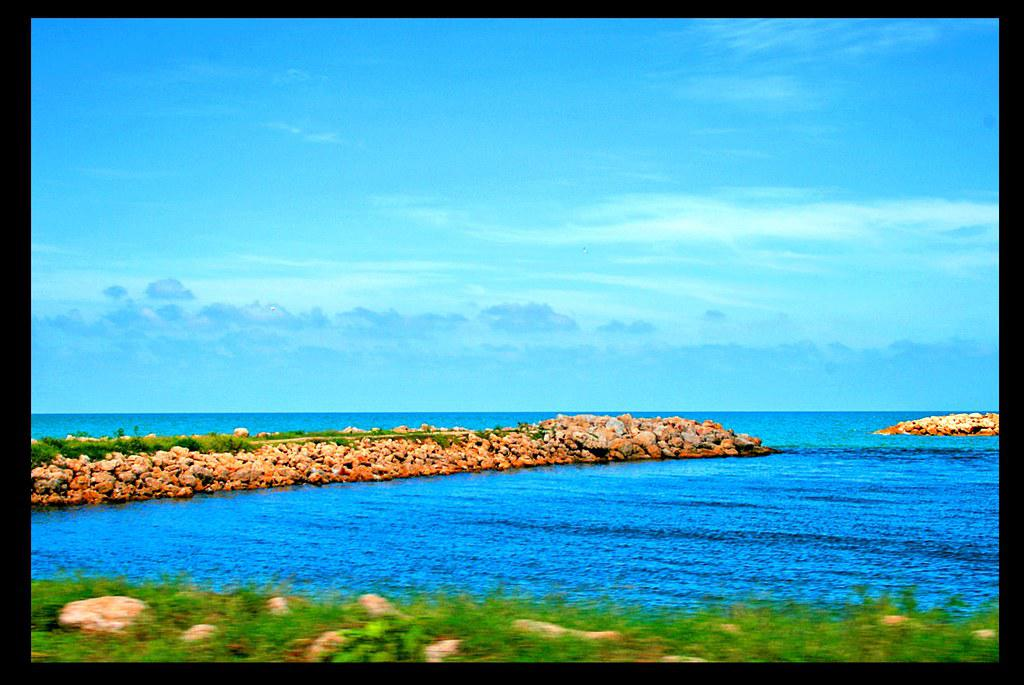
\includegraphics[width=10cm,height=5cm]{00000000_(5).jpg}\\ 	
							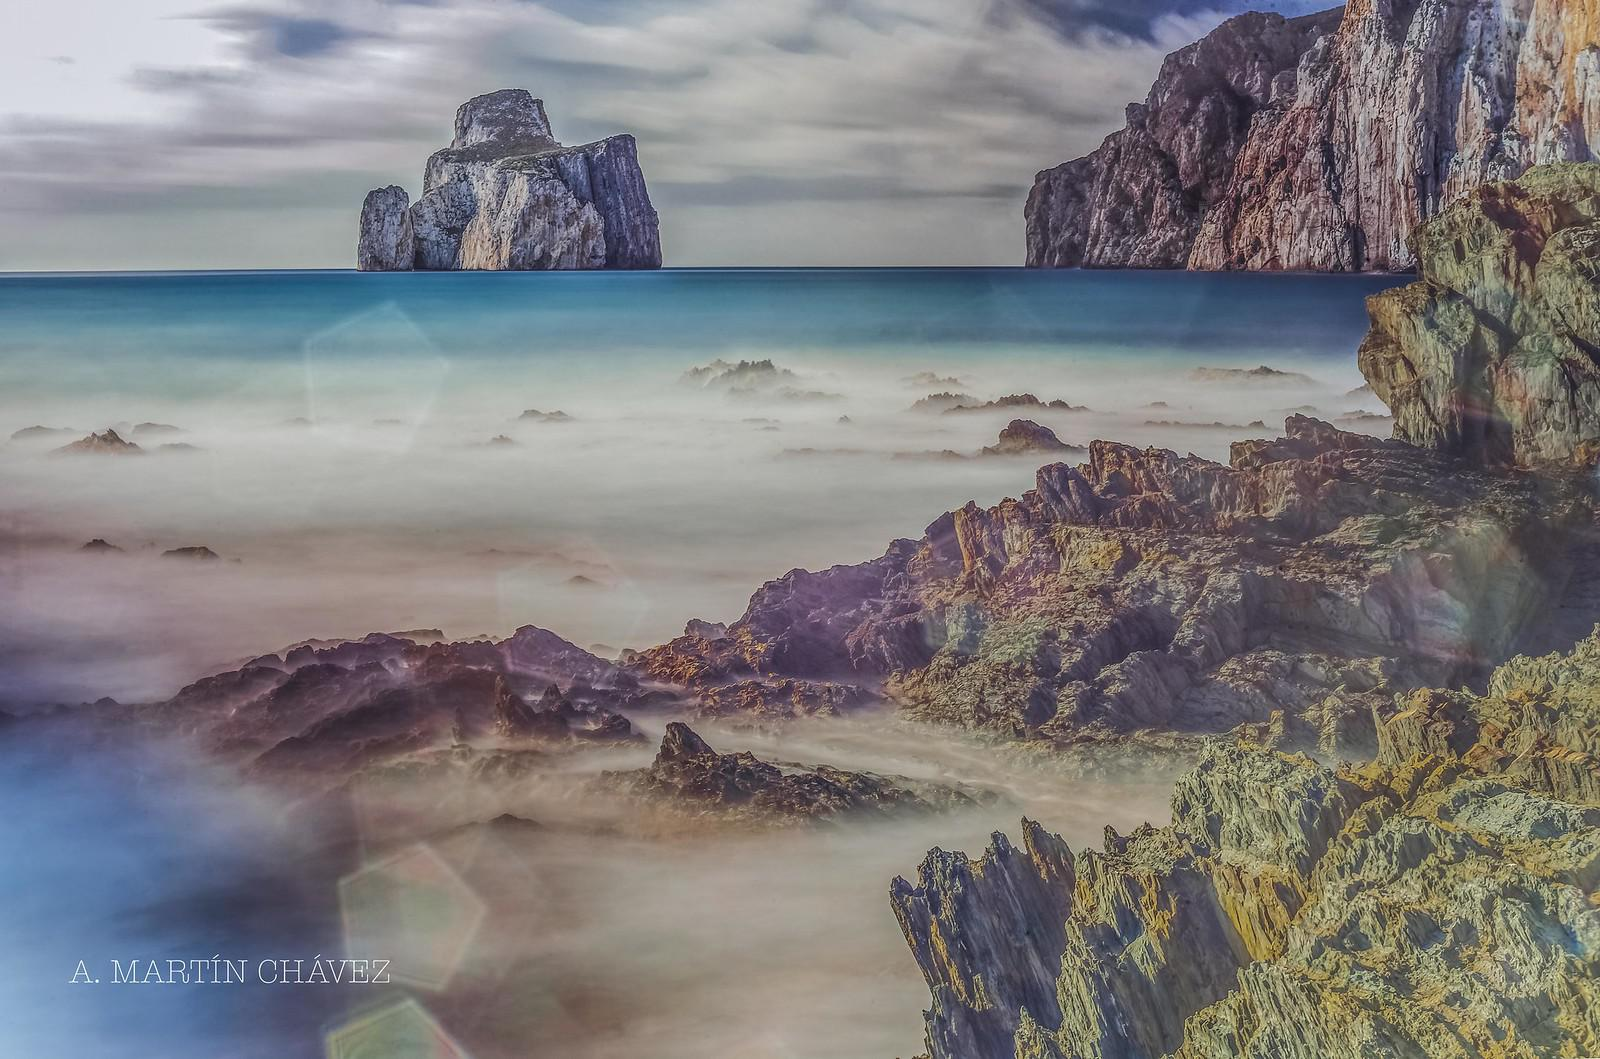
\includegraphics[width=10cm,height=5cm]{00000024_(2).jpg}
							
						\end{figure}

						
						
						\section{Beklenen Sonuçlar}
						10 haftalık bir süreyi kapsayan bu projede, Stable Video Diffusion modelinin temel prensipleri ve kullandığı teknolojiler (örneğin, derin öğrenme, difüzyon modelleri) araştırılarak benzer teknolojiler ve çalışmalar (örneğin, DALL-E 2,gail) ile karşılaştırılacaktır. Bu sayede, Stable Video Diffusion modelinin güçlü ve zayıf yönleri belirlenerek, bu modele benzer bir modelin geliştirilmesine zemin hazırlanacaktır.
						Proje kapsamında, modelin metin açıklamalarını doğru şekilde yorumlayabilmesi için gerekli veri setleri ve eğitim yöntemleri belirlenecek, farklı manzara türlerini ve farklı metin formatlarını desteklemesi için gerekli geliştirmeler yapılacaktır.
						Projenin tamamlanmasıyla birlikte, kullanıcının girdiği basit metinden manzara resmi oluşturabilen bir model inşa edilmiş olacak ve bu modelin farklı metin açıklamalarına ve parametrelere karşı test edilmesi, modelin oluşturduğu resimlerin kalitesinin ve çeşitliliğinin değerlendirilmesi ve modelin sınırlamalarının belirlenmesi gibi işlemler tamamlanacaktır.
						Son olarak, projenin kapsamını, kullanılan yöntemleri, elde edilen sonuçları ve gelecekteki çalışmaları içeren bir rapor hazırlanacaktır.
						\cite{wang2018assessment}
					
												\begin{figure}[h]
							\centering
							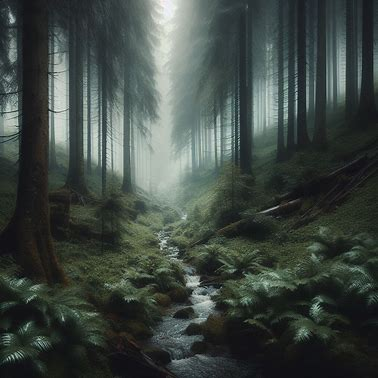
\includegraphics[width=15cm,height=5cm]{OIG4.jpg}
							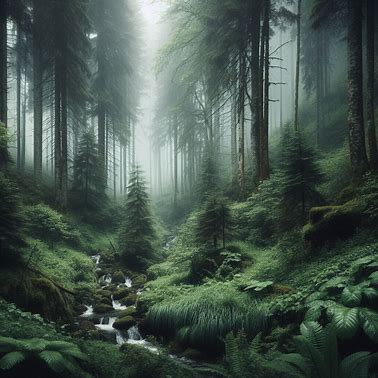
\includegraphics[width=15cm,height=5cm]{OIG4 (1).jpg}\\
						
							\title Powered by DALL·E 3 \\
						\end{figure}
						
					\newpage

			 		\textbf{GANTT Chart iş paketlerinin tanımı}\\
						\begin{figure}[h]
							\centering
							\includegraphics[width=15cm,height=5cm]{Şekil1.png}\\
							\title Şekil 1 \\
							
							\includegraphics[width=15cm,height=5cm]{Şekil2.png}
							\title Şekil 2 \\
						\end{figure}
						
						Şekil 1 ve şekil 2'de görebileceği üzere
						iş akış planı gösterilmektedir.
						\pagebreak
						

						\bibliographystyle{ieeetr} % We choose the "plain" reference style
						\bibliography{refs} % Entries are in the refs.bib file
						
							\newpage
							
							
							
							\pagenumbering{gobble} %Sayfa numaralandırması kalkıyor
							\pagenumbering{arabic} %Sayfa numaralandırmasını bu sayadan başlat
						

							
						
						\newpage
						
						
						
						
					\end{document} 